% Set a sane document class, 10pt font, and a report template
\documentclass[a4paper, twoside, openright, 12pt]{report}


% Import used packages
\usepackage{graphicx}
\usepackage{hyperref}
\usepackage{listings}
\usepackage{longtable}
\usepackage{lscape}
\usepackage{parskip}
\usepackage{color}
\usepackage{multirow}
\usepackage[lmargin=25mm,rmargin=25mm,tmargin=40mm,bmargin=30mm]{geometry}
\usepackage{setspace}
\usepackage{fancyhdr}

% Bibliographies
\usepackage[defernumbers=true]{biblatex}
\bibliography{slr-scbw/bib/bib}
\bibliography{bibliography}

% Use UTF-8
%\usepackage[utf8x]{inputenc}
\def \authors {Ken B\o{}rge Melhus Viktil and Martin Tobias Holmedahl Sandsmark}
\def \papertitle {An architecture for an agent playing StarCraft: Brood War}

% Meta-information for the PDF
\hypersetup{
pdfauthor = \authors,
pdftitle = \papertitle,
pdfsubject = {Pre-project for IDI},
pdfkeywords = {project, cognitive, architecture, starcraft, artificial
    intelligence},
pdfcreator = {LaTeX with hyperref package lol},
pdfproducer = {pdflatex}}

%opening
\title{\papertitle}
\author{\authors}

\begin{document}


\begin{titlepage}
\begin{center}

\vspace*{8cm}
\hrule height 1pt
\vspace{.5cm}
\huge{\papertitle}

\vspace{.5cm}
\large{\authors}
\vspace{.5cm}
\hrule height 1pt

\vspace{6cm}
\end{center}
\normalsize
\begin{table}[!h]
\begin{tabular}{ll}
\multirow{4}{*}{
\includegraphics[width=20mm]{graphics/logo.png}} & \\
& Department of Computer and Information Science \\
& Faculty of Information Technology, Mathematics and Electrical Engineering \\
& Norwegian University of Science and Technology \\
\end{tabular}
\end{table}
\vspace{.5cm}
\begin{center}
\today
\end{center}
\end{titlepage}
\pagenumbering{roman}
% Insert an empty page
\newpage
\thispagestyle{empty}
\mbox{}

\begin{abstract}
We present an overview of the most important aspect of the game StarCraft as
pertaining to designing a computer program that can play it using artificial
intelligence methods. We then present existing approaches to agent architectures
for playing StarCraft, and an analysis of these. We also present an overview of
an established architecture for simulating cognitive models, which has earlier
been used in robotics and first-person shooter games. Finally we present our own
architecture for an agent playing StarCraft, inspired by the aforementioned
cognitive architecture.

This we hope can be used for the final project with the goal of developing an
agent that can represent the Norwegian University of Technology and Science in
an international competition against other agents.
\end{abstract}


\pagenumbering{roman}
\tableofcontents

\listoffigures

%\listoftables

\pagenumbering{arabic}
%!TEX root = main.tex

\chapter{Introduction}

\section{Background and motivation}

\subsection{The Problem}
In 2003 Michael Buro published an article where he requested more artificial
intelligence research in the domain of real-time strategy
games.\cite{buro2003real} Before this, a lot of research was focused mainly on
turn based, real-time board games, like chess and checkers. A lot of
progress has been done in these fields to the point where they are now able to
beat top level human players in a real-time match. \cite{campbell2002deep} But
these games are both deterministic and fully observable, whereas real-time
strategy games usually are only partially deterministic and partially
observable, which makes for much more interesting problems.

In the wake Buro's call to arms more work has been invested in this area, and
several platforms for RTS research has been used. One platform that has been
used a lot is Wargus\cite{wargus}, a clone of Blizzard's Warcraft 2, where they
created a Lua-based AI scripting language for efficient artificial game-playing
agent creation. But this game had quite severe limitations on individual
management of units, so in recent years StarCraft: Brood War has been getting a
lot more attention as a platform for experimenting with game playing agents.
Several competitions are held each year where implemented AI agents can
compete with each other and measure their performance. But even though a lot has
happened with the field in recent years, Starcraft agents still have ways to go
before they can measure up to a human player.\cite{eisbotvsfong}.

Simply winning is however not always the goal, most game-playing artificial
intelligences are made to be realistic and engaging to compete with, so in many
situations simply playing well is not enough. According to Arrabales et
al \cite{arrabales2009gamechars} it is still more realistic and engaging to be
playing with other humans than with synthetic agents. So to attempt to lessen
this gap, it could be interesting to make synthetic agents play more human-like,
and to do this one would probably want to look into more biologically inspired
methods, for example inspired by cognitive architectures.

Cognitive architectures have proven to lead to human-like behaviour and choices
in both games\cite{arrabales2009gamechars} and general problem
solving\cite{franklin2003interacting}, and the logical conclusion therefore
seems to be to try to apply these models to StarCraft.

\subsection{StarCraft: Brood War and BWAPI}
StarCraft is one of the most popular real-time strategy games in the world. It
was developed by Blizzard Entertainment, and in 1998 they released the expansion
pack Brood War. The expansion pack included new maps, units and upgrades for
each of the races in the game.
 
Since its release it has been widely played in professional tournaments, as well
as been used extensively in research on artificial intelligence, thanks to the
BWAPI project which is a free software project aimed at developing and
maintaining an API, named BWAPI, for creating artificial intelligence modules
for Brood War. In addition, this API is the basis for several yearly
competitions where people can submit AI bots that will be pitted against other
bots to measure their relative performance. This has led to a large number of
AIs being developed of various degrees of complexity and novelty, both from
researchers and hobby developers. 

\subsection{The project}
In this project we will familiarize ourselves with the game StarCraft: Brood
War, and what challenges that presents when creating a computer program that
will play the game. We will identify the different aspects of a StarCraft game
that are important to solve in order to create a good game-playing agent, and
also look at how other researchers have solved these problems in their agents.
Ultimately we will select and define an architecture for our system that will
have an modular approach in order to support easier collaboration when
implementing the system, based on a cognitive model.

In order to get a good overview of existing solutions and map the current state
of the research into this field, we will perform a structured literature review.
This will give us a good overview of the theory behind the state of the art
when it comes to our research problem.

So our project is divided into three main parts:
\begin{enumerate}
  \item Identify the most important aspects of a StarCraft match.
  \item Research existing solution and theories, using a structured literature
review.
  \item Design an architecture for a modular StarCraft playing computer
program, based on a cognitive model.
\end{enumerate}

\section{Contributions}
For the structured literature review we collaborated with Magnus Sellereite
Fjell, Stian Veum M{\o}llersen, Tobias Laupsa Nilsen, J{\o}rgen B{\o}e Svendsen,
Espen Auran Rathe, Aleksander Lun{\o}e Waage, {\O}ystein Samuelsen, Finn Robin
K{\aa}veland Hansen, Dag-{\O}yvind Tornes and Jan Eriksson.

We are also grateful for the feedback and cooperation with everyone on the
\#BWAPI IRC channel on QuakeNet, and especially Adam Heinermann who is also a
lead developer on the BWAPI project.

We would also like to thank our supervisors; Helge Langseth, Anders
Kofod-Petersen and Pauline Haddow.

\section{Report Structure}
This report is structured into four chapters:
\begin{itemize}
\item Chapter 1: \textbf{Introduction} \\
This chapter describes the motivation and goal of the project as well as who contributed and the general structure of the report.
\item Chapter 2: \textbf{Theory} \\
This chapter is threefold. First it presents some theory on StarCraft in
general, how the most important mechanics works and the difference between the
available races. Then we go over the state of the art when it comes to agents
who play StarCraft, both how the problems they solve are partitioned, as well
as how some of the most important agents today are architected. Lastly we go
over some background on the current state of cognitive research and models
utilizing this.
\item Chapter 3: \textbf{Results} \\
Here we present our results; our novel architecture for an agent for playing
StarCraft: Brood War based on the cognitive models we explored earlier.
\item Chapter 4: \textbf{Evaluation} \\
Here we summarize and evaluate the work presented in this report.




\end{itemize}
%!TEX root = main.tex

\chapter{Theory}

%!TEX root = main.tex

\section{Starcraft}
\label{sec:starcrafttheory}
\begin{figure}[h!tb]
\centering
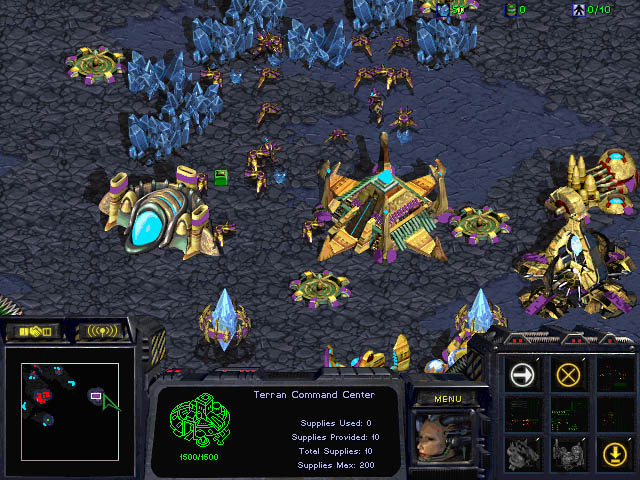
\includegraphics[scale=0.5]{graphics/scbw.jpg}
\caption{Star Craft Brood War}
\label{fig:scbwIntro}
\end{figure}

Starcraft is a military science fiction real-time strategy developed by Blizzard
Entertainment in 1998.\cite{starcraft} The game has a single-player campaign,
but it is most famous for its one vs. one multi-player where the goal is to
defeat an opponent on the battlefield, using one of three distinctive races;
the earth-originated Terrans, the advanced Protoss or the hive-minded,
insectoid Zerg. Starcraft Brood War is an expansion pack for the original
Starcraft that introduces new units, upgrades and maps. 

A typical multi-player game starts with each player choosing their race and the
selection of a map to fight on. Each player are then spawned in one of
several potential start locations. If the map has more than two start
locations, they don't know where the enemy spawns and will have to go look for
them. Each player is given a foundation building and a few workers at the
beginning of the match, and how the rest of the match then unfolds are now up
them. A match consists of gathering resources and securing one or more bases in
order to produce units for an army that can be used to defeat the enemy. Victory
in the match is achieved by killing all of the opponents structures or forcing
them to concede.

The resources in the game are minerals and gas. Minerals are mined from mineral
formations that are found in each base location, and placing the foundation
building close to them is important so the workers do not have to move to far
when they collect minerals. Gas is extracted from geysers that are found next to
the mineral formations, but in order to harvest it a player must build a
specific structure on top of the geyser. Afterwards, workers can collect gas in
the same way they collect minerals. Each base location has a limited amount of
minerals, and in order to continue to acquire minerals a player must expand to
another base by building a new foundation building at that location. Taking
several bases at the same time allows for increased income and greater unit
production. But there are a limited amount of minerals on the map which will
force a match to end in a reasonable amount of time (towards the end players
won't be able to resupply their armies). Gas on the other hand never runs out,
but after a certain threshold of gas collected from it, gas will be collected at
a reduced rate of 1/4 of the original one.

Starcraft is on the surface a very simple game, it has only three different
playable races, a handful of different buildings and units, and with goals that
are relatively simple to comprehend. But once you start analyzing the game, the
reality is quite different. The Brood War expansion pack was released back in
1998, and the game has been played at a competitive, high level since then and
all the way up to today. And the metagame\footnote{Metagame is a description of
the part of the game that transcends a single match, for example popular
strategies, tactics, counters to these, at a given time.} has evolved during the
entire lifespan of the game and is still changing today with new tactics showing
up from tournament to tournament. \cite{starcraft}

When playing at a high level you are working with really small windows of
opportunity, often called timings. And it is these timings that enable a game
with what should in theory be simple elements to have such complex and evolving
strategies. The effectiveness of an attack on the enemy bases can be decided by
the presence of a single important unit, so if this unit is produced 20 seconds
to late the attack could have crushed the defending army and started killing
buildings by the time that unit is finished. When playing with so small margins
every little change can have massive consequences on the outcome of the match,
and this creates the high level of dynamic play that Starcraft is known for.
 
\subsection{Macro and Micro}
Macro-management and micro-management, henceforth referred to as \textit{macro}
and \textit{micro} respectively, are the two concepts that you have to master
in order to play Starcraft, or any other RTS, at a successful level. These
concepts incorporate everything from low level control of units to the high
level strategy and tactics used in a game. And finding a good balance between
them are one of the main challenges about playing RTS games for human players.
Micro is the ability to control individual or group of units in an efficient
way. Having better micro than your opponent enables you to win fights where you
have an equal or even outnumbered army. Good micro enables you to 
compensate for poor in-game AI/path finding by individual control of the
units, this also allows you to save more units that are taking heavy fire and to
focus down important targets in the enemy army. Macro is the ability to produce
units and construct new buildings at the appropriate times. Good macro means you
are always producing something with your buildings and and that you expand or
increase your production capacity at appropriate times when you have the
resources to support this. The player that has the best macro usually have the
biggest army when the time to battle comes. While it is best to have both great
macro and great micro, this is usually not possible, so players have to choose
where they spend to use their attention. Because good macro means you will have
a better economy and more units it is generally agreed that macro is more
important then micro, though it is important to have a good balance of both in
order to play at a high level.

\subsection{Supply}
In Starcraft there is always a limit to how many units a player can have at a
given time. This is called supply for terran, control for zerg and psi for
protoss. They function the same way for every race, so most people just call it
supply no matter what race they are talking about. Each race has a building or
unit that can increases their possible supply count up to a maximum of 200.
Terran has a building called the supply depot, protoss has a building called a
pylon and zerg uses a flying unit called an observer. More powerful units have a
larger supply demand then basic units, so you you can have less of them before
you run out of available supply. It is therefore important to find a balance
between basic and advanced units that gives you an good sized army but also with
powerful units. Because zerg have more basic units, and protoss have more
advanced units it is very normal for a zerg player to have a greater army size
and the protoss to have a smaller army but with more powerful single units.
 
Supply blocked is what happens when a player can't create any more units because
he has reached his maximum supply. This can happen when a player forgets to
build more supply buildings/units as he is creating new units, or an enemy
destroys one or more of the buildings/units that increases the supply count.
Being supply-blocked can have big consequence as it gives the other player an
edge to exploit because you can't create any more units until the supply is
increased by creating new supply buildings/units. This small edge can be just
what the enemy needs to pull ahead in the game and get a victory. Because of
this players will often launch hit and run attacks that are aimed at supply
blocking the opponent.
 
\subsection{Fog of War and Scouting}
Starcraft is a game with imperfect information, meaning you do not see
everything that is happening on the map. The map is covered by a \textit{fog
of war} that hides what is happening. Any unit or structure that you own reveals
an area around itself where you can see everything. Because of this scouting
becomes a very important aspect of playing Starcraft. Scouting means sending a
unit out to places on the map where you don't know what is happening, the most
important area being the opponents base. But also to make sure he has not placed
buildings or hidden armies someone else on the map. Early game it is very common
to send a worker unit out to look around the opponents base in order to gather
information on what he is doing and what strategies he is working towards so
that you can counter this. This also means that denying the opponent scouting
information at critical stages in the game is an important aspect, for instance
hiding that you are building air units so that you can launch a surprise attack
that will catch them unprepared. Other ways to exploit the fog of war is to
create hidden expansions\footnote{Extra foundation buildings used to generate
additional income from other mineral patches or gas geysers.}, or hide important
buildings so it is more difficult for your enemy to figure out what strategy you
are going to use. 

\subsection{Races}

\subsubsection{Terran}

Terran are the human faction of StarCraft, a futuristic version of man today.
They are known for high adaptability with a good variety of defensive and mobile
armies. They are best known for their mobile biological armies, or their slow
moving turtling tech(tanks) armies that slowly creeps across the map and secures
section by section. This versatility makes them a great class with a lot of
different possible strategies and combinations that can be effective.
 
The Terran worker is the Space Construction Vehicle (SCV). This unit can gather
minerals, build buildings and, unique for the Terran race, repair other
mechanical units or buildings. When constructing buildings the unit has to work
on the building from the initial placement to the building is complete, meaning
it will be unable to perform other action in this time, and can be attacked. If
the SCV halts construction or is killed, the building will have to be canceled
or finished by another SVC. Like mentioned before it can also repair mechanical
units like tanks if they have taken damage, but to perform this action they have
to be pulled from other tasks like mining minerals so it is a two edged sword.
Terran buildings will slowly self destruct if left at low health, so it is
important to repair them if they have taken significant damage.
 
Terran buildings also have a unique feature in that they can lift of the ground
and fly around after being constructed. They can then land in a new location and
continue production of units or upgrades. Some buildings can also create add-ons
that unlocks new units and upgrades for that building. Terran also have a unique
building in the bunker. This a a defensive building where  biological units can
seek refuge while still attacking, but from a fortified position that protects
them from damage. The bunker has to be taken out before the units inside can be
damaged and killed. While being useless on it's own, the building can be a death
trap when filled with infantry. The bunker can also be repaired by an SCV, like
any other Terran building, so the SCVs have to be a priority for an attacking
army before they can destroy the bunker.
 
The health regeneration mechanics for the Terran race are twofold. The medic is
used to heal biological units after they have suffered damage in battle (they
can also heal other medics, but not themselves). Mechanical units can be
repaired by pulling SCVs, for example from mining, and using them to repair the
unit. SCVs can also be effective to use in combat as they can repair the unit
while it is taking damage, and several SCVs can repair the same unit at the same
time for an increased regeneration rate.
 
\subsubsection{Protoss}
The protoss are a technologically advanced alien race that rely on psionic
abilities and cybernetics in battle. Because they are the most technological
advanced race in StarCraft they are known for their raw power. With powerful but
expensive units they can crush their opponents on the battlefield even if they
are outnumbered army because of superior firepower.

The protoss worker is called a probe, and is like the SCV used to gather
minerals and build buildings. Protoss buildings are not constructed, but warped
in from their home planet, so a probe only needs to place a warp beacon where
the building should be placed and then it can return to mining minerals while
the building warps in by itself. This allows the use of one probe for
construction of several buildings at basically the same time, and then it can
return right to mining. This can allow an protoss player to setup remote
expansions in a short time with a single probe. 

In contrast to the terran race the protoss can't just build buildings anywhere,
they have to place them on a power grid generated by a pylon, the protoss supply
building. Pylons also power buildings, so if an enemy takes out all the pylons
around some production building it can no longer produce any units or research
upgrades. The player will then have to build new pylons to power up the building
again before he can continue production. 

Special for protoss units and buildings are that they have energy shields that
protect them against damage and recharges to full strength over time. In order
for an enemy to damage a protoss unit, it has to first deplete the shield that
protects it, only then can they proceed to damaging the unit itself. For an
enemy it is therefore important to finish of the unit when it's shield is fully
depleted or it will regenerate to full strength. 

\subsubsection{Zerg}
The zerg are not actually a race of its own, but rather a collection of very
different creatures and races that have been assimilated and united under a
central intelligence called the Overmind. Striving for power, they have been
selectively evolved towards being very effective killers. Technologically they
are far behind the other races, but they make up for this with a big army size
and superior biological properties. 

The zerg worker unit is called a drone. When constructing a building a drone
will ``sacrifice'' itself and mutate into the building. This means that for
every building that the player constructs he loses a worker. In every other way
they behave just the same as the worker units for the other races. For every
race the worker unit is produced from the foundation building, for zerg this is
the hatchery. But for zerg every other unit is also created from the hatchery,
and any unit buildings that are constructed only unlocks the possibility to
create that unit from the hatchery. This is because zerg have a special game
mechanic called larva. These special non-controllable units are produced by the
hatchery over time, up to a maximum of three at a given time, and they can be
morphed into another zerg unit that is unlocked (units they can be morphed into
depends on what buildings the zerg player has built).

Similar to protoss the zerg can't just build buildings anywhere, because the
buildings are biological they require nourishment to function, and have to be
built on creep. Creep is produced by the Hatchery and Creep Colonies and then
radiates outwards from these onto any fertile ground in the area. The Hatchery
is the only building that can be built without creep, as it produces its own
nourishment. 

Zerg units and buildings have a unique ability to regenerate lost health over
time if left alone. This means an attacker should finish off an attacked unit or
it will come back with full health after a while. This also makes tactical
retreats much more important for the zerg players, as they can then rest their
army to allow them to regenerate back to full health after taking damage in a
battle. Burrowing is also a unique ability for the zerg units, and has great
synergy with the health regeneration ability. This allows them to burrow in the
ground to get out of harms way, and here they can regenerate health without
worrying about taking damage. This also allows for ambush tactics by burrowing
armies and waiting for the enemy before launching a surprise attack. It can even
be used to gain map control by burrowing units in strategic places to scout that
area. Only using some form of detector can the enemy see and attack units that
have burrowed. 

\subsection{BWAPI}
The Brood War Application Programming Interface (BWAPI)\cite{bwapi} is an open
source C++ framework project for creating AI modules for Starcraft: Brood War.
BWAPI is a third party ``hack'' of Starcraft: Brood War to allow programmers to
retrieve and send information to the game at real-time. The API provides the
programmer with information about the game state and the individual units, as
well as allows them execute actions similar to what a normal player would be
able to perform. 

There are a two different ways to ``inject'' an agent into StarCraft; it can be
made as a module that gets loaded into StarCraft or as a standalone process that
communicates with BWAPI through a shared memory area, a client-server approach.
What method to use depends on several factors, but mainly what language that
will be used. Because BWAPI (and StarCraft itself) is written in C++ the module
that gets ``injected'' have to be in the same language, but the client-server
approach much more easily enables other languages to be used as the client side
is independent and can be written in any language that has a port of the BWAPI
protocol. This includes several languages such as Java, C\#, Python and F\#.
The API also supports several degrees of accessibility, meaning you can play a
game as a normal real player would with limited information, or you can start a
game that is fully observable. The later is mainly of academic interest, where
you want to test an AI that requires a fully observable environment.

The API provides extensive and detailed information about the game state,
basically anything a player can see in a game is also available though the API.
Some examples of this are unit locations, production times, available
structures, cost of buildings and units. In some cases the API even provides
additional information that is not available to a human player in the game, this
can be the exact unit speed and the damage and armor of a unit. This is
information that a player usually learns outside the game, but for an AI agent
it makes it easier for the developer, as a lot of domain knowledge can be
retrieved from the API as apposed to having to bundle this in every agent. 

\subsubsection{BWSAL}
BWAPI Standard Add-on Library (BWSAL)\cite{bwsal} is a project that have created
several add-on to the standard BWAPI. The project aims to be a foundation for
creating AI agents with BWAPI. The main parts of the Library are managers that
handles a lot of the boiler plate code that is required to get a functional
agent with BWAPI. Features like finding available locations where one can
construct a building, basic control of units and workers, scouting and build
order managers are available. A lot of this code would be quite similar and time
consuming to create for each AI agent, so using the add-on library one can much
easier get a working agent up and running and the developers can start focusing
on their main priorities. 

\subsubsection{BWTA}
The Brood War Terrain Analyzer (BWTA)\cite{bwta} is another add-on for BWAPI
that is used for analyzing the terrain in Starcraft maps. BWTA calculates
regions, choke points and base locations on the given map. The calculations are
done before the match, and the results can then be accessed and used by the
agent as it sees fit.  
\section{Artificial Intelligences for StarCraft}
There have been a handful of relatively successful AIs for StarCraft.

\subsection{In-game AI}
The in-game AI is considered not very good.

\subsection{Berkeley Overmind}
This is considered one of the best AIs, not perhaps because it is very complex,
but because it has a solid ``cheese'' and has been well-tweaked.


%!TEX root = main.tex

\section{Architectures}
Classical games like chess or tic-tac-toe are usually ``solved'' by AIs using a
single approach and searching through a single tree of game states, though
usually by optimizing the search and tree in various ways.

In comparison most approaches to AIs playing real-time strategy games usually
have to use domain knowledge do further subdivide the problem of playing the
game, because of the fine-grained simulations involved, and the various levels
of abstraction that is needed to get a successful AI. And especially when
approaching the way humans think about a problem more complex architectures
are needed.

\subsection{Decomposition of problem}
Michael Buro in his 2003 call for research \cite{buro2003real} identified six
important sub-problems in real-time strategy games that he said would be
interesting for AI research to focus on:

\begin{description}
  \item [Resource management.] To be able to build up an army one needs to gather
    resources, and the balance between gathering resources (by creating workers),
    building an army and evolving through the technology tree is an important
    part of the macro/high-level strategy.
  \item [Decision making with uncertainty.] Because of fog of war, there is a
    high degree of uncertainty involved in the decision making. Therefore the AI
    needs to create hypotheses and act according to them, and should scout to
    confirm these.
  \item [Spatial and temporal reasoning.] Analyzing and predicting spatially as
    well as temporarily. Identifying choke points and predicting outcomes and
    utilities of actions it takes are some obvious applications.
  \item [Collaboration.] In most RTSes it is possible for players to ally, and
    how to share intelligence and coordinate attacks is a challenging problem,
    though maybe not as interesting yet.
  \item [Opponent modelling.] Learning from the opponent is an important skill,
    and exploting the weaknesses of your opponent is an important aspect of
    human-level playing.
  \item [Adverserial real-time planning.] Abstracting away micro-level
    management to allow for more efficient search in the game state-space, and
    translate the found solutions back, is an important problem to solve.
\end{description}

A lot of research as been done into AIs for RTSes since this, however, and the
list might be a bit outdated. For example, one important aspect of most AIs
today is the micro-management of units, trying to maximize the utility of them 
(maximizing output of resource gatherers and damage dealt by offensive units,
for example).

Another important problem that is under-valued by the above list is learning
from existing knowledge, like learning build-orders from replays of games played
by humans (or other bots, though the utility of that might not be substantial).
This can be integrated into several of the items above, for example the decision
with uncertainty by statistically inferring the most probable states by
learning from earlier games.

A more general and simplified breakdown of the problem of playing Starcraft can
be found in Ben Weber's presentation from the AIIDE 2010 StarCraft AI
Competition:\cite{weber2010aiide}

\begin{description}
  \item [Managing economy] is the same as the resource management mentioned
    above, and is about getting a steady income.
  \item [Expanding the tech tree] to get more powerful and varied units.
  \item [Producing units] is perhaps one of the most complex parts. This
    involves both buildings and movable units, defensive and offensive.
  \item [Attack opponent] usually is not a very explicit action, but can still
    be pretty complex, since one needs to evaluate its own state against what
    it knows about the opponent to know when to attack, and where. This point
    also involves micro-management, which has received a lot of attention from 
    authors of AIs that have ranked highly.
\end{description}

Solving all of the aforementioned problems by themselves are what is the focus
of most research today, but another important problem is tying all of these
solutions together again. This is perhaps one of the most basic, but important,
aspects of the architecture. There are several different ways of doing this,
and some of the most common one is simply sharing a large amount of information
between sub-units in the architecture (for example a black-board based
architecture), or simply having a well-defined graph hierarchy where decisions
are propagated.

\subsection{Architectures of current state of the art Starcraft AI}
Each year there are several big AI conferences that run Starcraft AI RTS competitions. The the two biggest are held at the Computational Intelligence in Games conference(CIG)\footnote{\url{ttp://ls11-www.cs.uni-dortmund.de/rts-competition/starcraft-cig2011}} and the AI and interactive digital entertainment conference(AIIDE)\footnote{\url{http://www.starcraftaicompetition.com/}}. Here most the the state of the art bots come together to measure their strength compared to the other bots. Most of the time playing vs a real player is not something that the bots can be very effective, so these competitions becomes the only real way for researchers and developers to test their AIs and get some reasonable feedback on the level of play they are capable of.

\subsubsection{BTHAI}
BTHAI utilizes a multi-agent approach to create a system with high levels of modularity. Each unit and building is represented as an agent that extends a more general version of that agent type. So every building is a subclass of a structurAgent, and every unit is a subclass of an unitAgent. These again extend a baseAgent, and this creates a hierarchic structure where agents of a similar type can share logic for behavior and strategy, but supports the option of extending the agent in order to customize and specialize the behavior of that specific agent. 

For higher level tasks with as tactics, exploration and building the bot uses managers. The managers maintains all the agent objects for the different units that the bot controls. Managers also act as an information provider for the agents so they can access data and statistics about the current state of the game. For instance how many units that an attacking force consists of, and how many are defending the base etc. 
There are also an exploration manager, that handles everything related to exploration, where enemy units have been discovered and predictions about where they will move. A build planer decides what order buildings will be constructed in, and squad commanders handles higher level tactics for a group of units, like attacking or retreating. These managers also have an hierarchic structure, so that they can be extended in order to create a more specialized manager, like a race specific build planer. 

The creation of agent instances are the responsibility of an AgentFactory. This factory makes sure that the correct agent is created for a given unit and that if there exists a specialized agent type for that unit the correct one is created and not a general agent. 

For movement of individual units the bot utilizes a potential field implementation. Agents can decide depending on the situation and the need for precise movements if they want to use the built-in starcraft path-finding or the potential field module. 

Figure \ref{fig:bthaiarch} shows a general overview of the architecture used in BTHAI

% TODO: maybe clear page here if that fits when report is done. 

\begin{figure}[h!tbp]
\centering
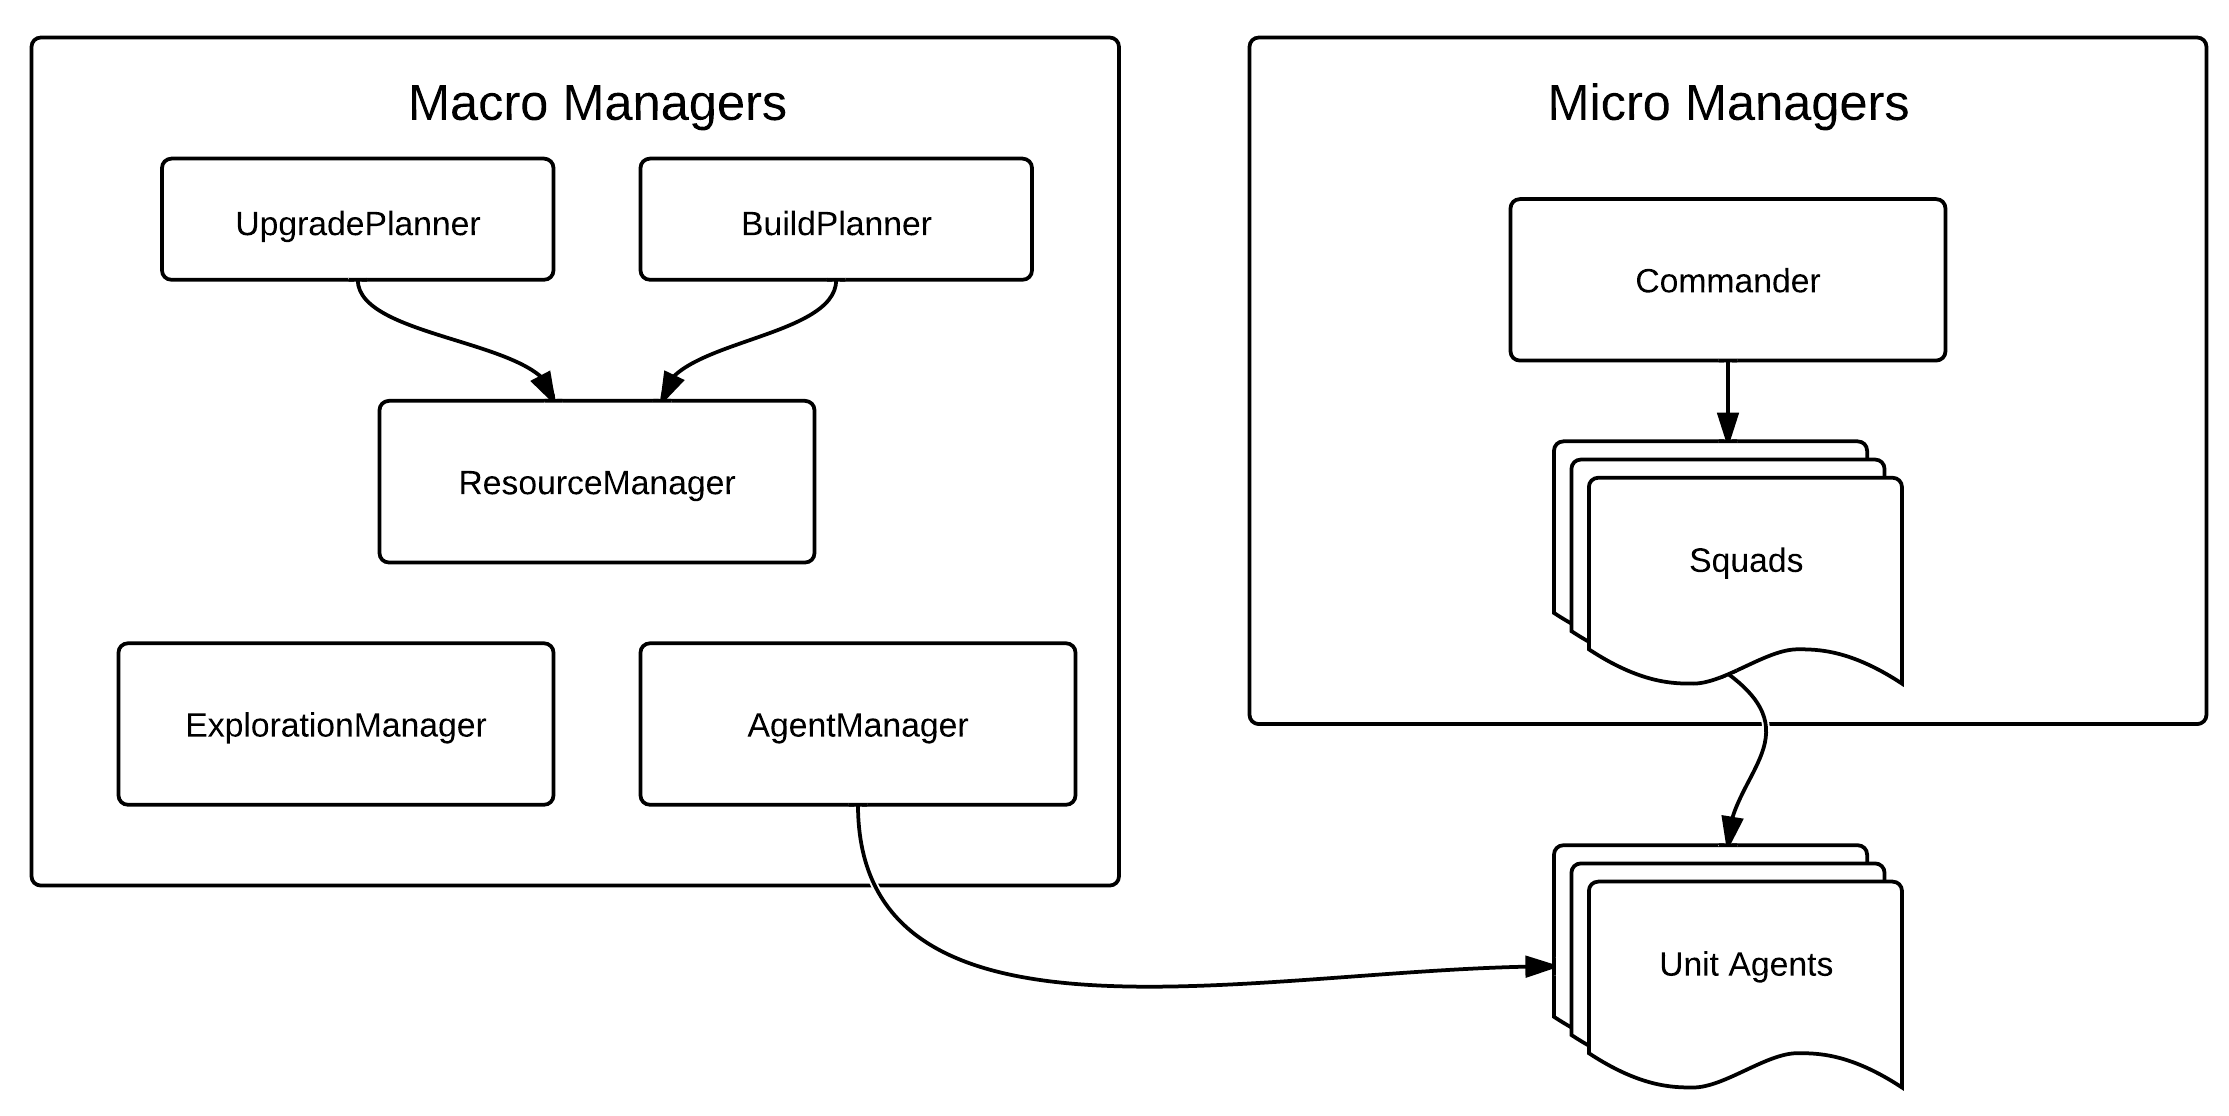
\includegraphics[scale=0.8]{graphics/bthai.png}
\caption{BTHAI general architecture}
\label{fig:bthaiarch}
\end{figure}

\subsubsection{BroodwarBotQ}
BroodwarBotQ has taken a more divide-and-conquer approach to the higher levels of macro control then BTHAI. Meaning it has separate agent types for the different tasks that a starcraft game consists of. Worker manager, bases manager, production manager, and construction manager are some of the macro oriented agent types that this bot utilizes. None of the managers controls are orders any of the others around, so the problem of playing starcraft is divided into subtasks that each has a manager that should solve them. But some of the subtasks are not entirely independent, so in order to resolve conflicts between the modules BroodwarBotQ uses a arbitrator. This also acts as a mediator between the macro and micro layers of the architecture. 

For this bot unit control is realized using Bayesian units that strives for completion different goals as ordered by an goal manager.\cite{synnaeve2011bayesian} One of the main goals for the author of BroodwarBotQ was improve the intelligence of starcraft bot, mainly the ability to predict and change strategy based on what the opponent is planing. So achieve this they have estimators that based on data extracted from starcraft replays using Bayesian models, tries to predict what the opponent are doing and planing and tries to adapt its own game play according to countering that. 

% TODO: maybe clear page here if that fits when report is done. 

\begin{figure}[h!tbp]
\centering
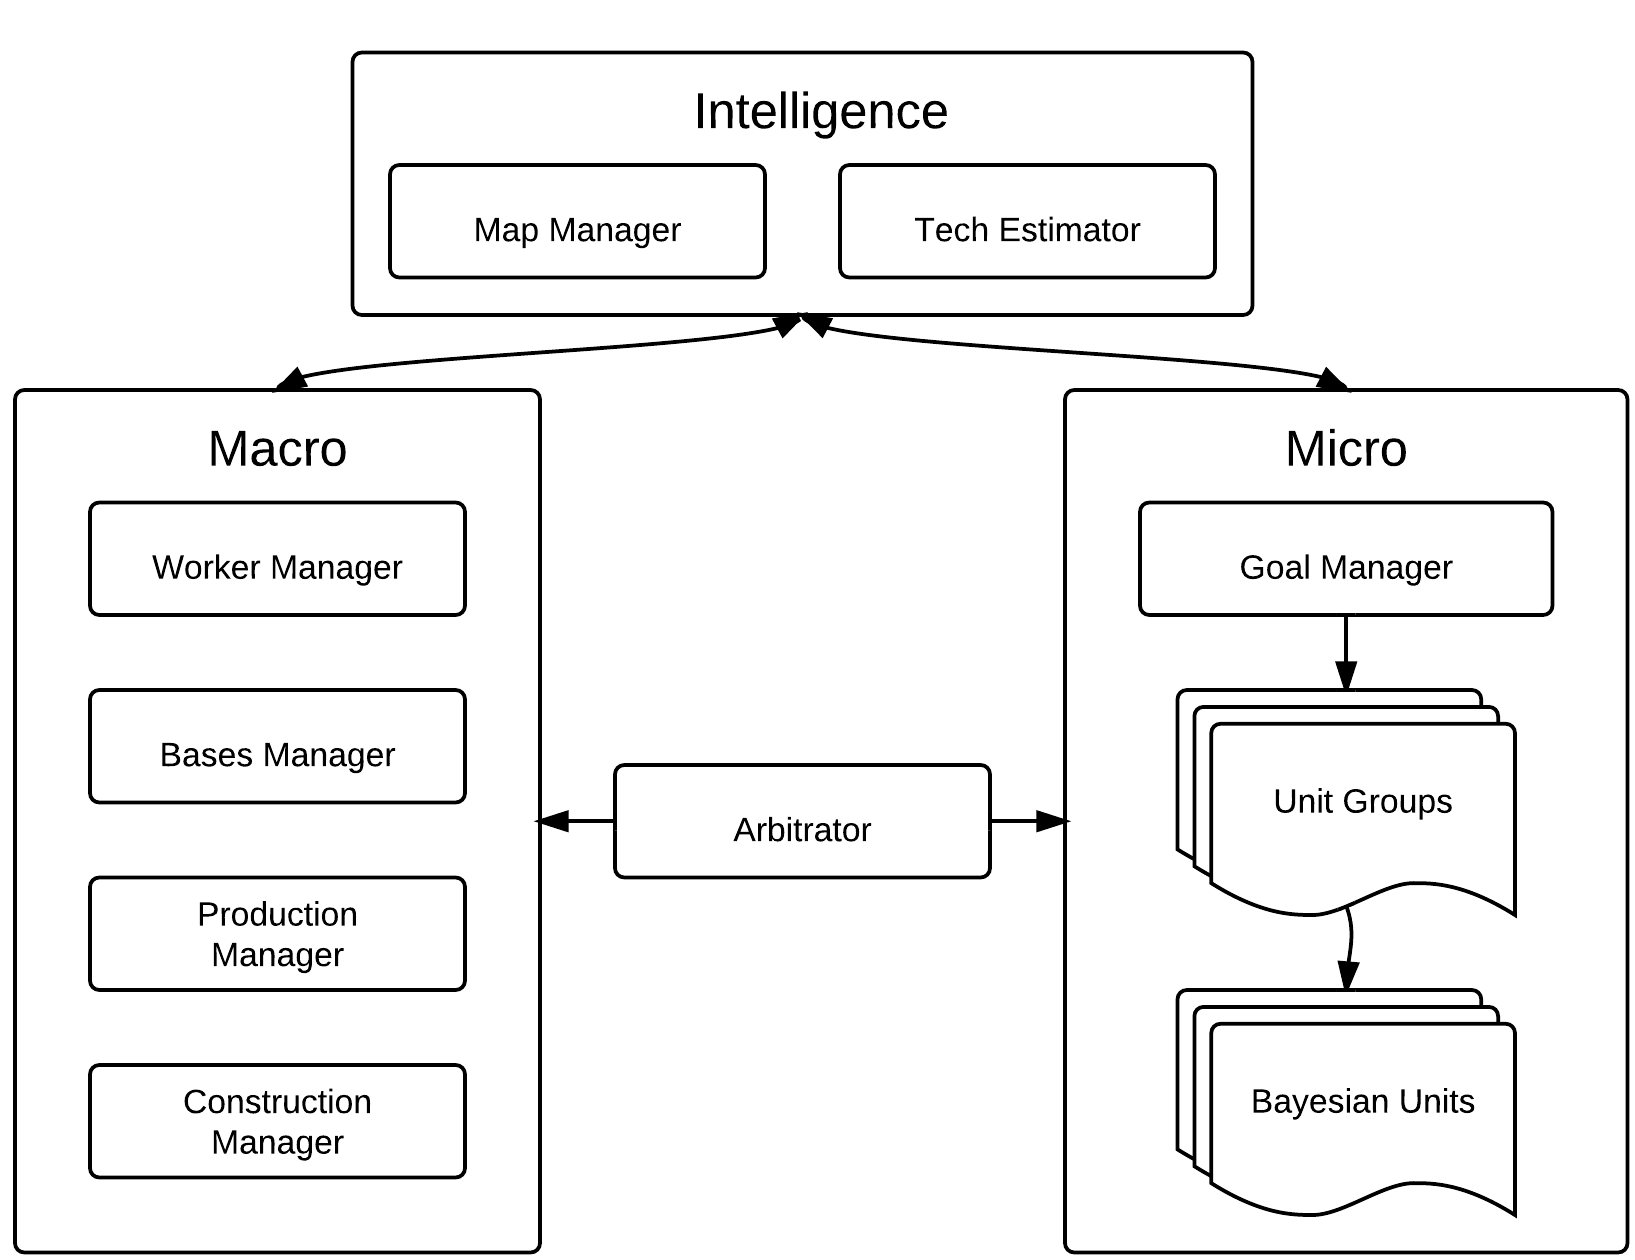
\includegraphics[scale=0.8]{graphics/bbq.png}
\caption{BroodwarBotQ general architecture}
\label{fig:bthaiarch}
\end{figure}

\subsubsection{Skynet}
Skynet uses a more hierarchic approach then most of the other bots, where it has divided its decision making into three different layers. Where higher level modules issuing commands to the lower level modules. The strategy layer at the top manages build order strategies that it gives commands to the tactics layer underneath to execute. The tactics layer contains all the managers that controls all the different aspects of the game, like resource management, scouting and macro management. All this managers outputs tasks that have to be completed and sends them to the task manager in the last layer. In this task layer each of the tasks in the queue will be given to a specific low level module that knows how to execute it. This is the only place where commands are sent from the bot to Starcraft. In addition the bot has a series of situational analysis modules that that continuously analyses the state of the game, and gives input back to the decision making layers when it identifies something that needs focus.

% TODO: maybe clear page here if that fits when report is done. 

\begin{figure}[h!tbp]
\centering
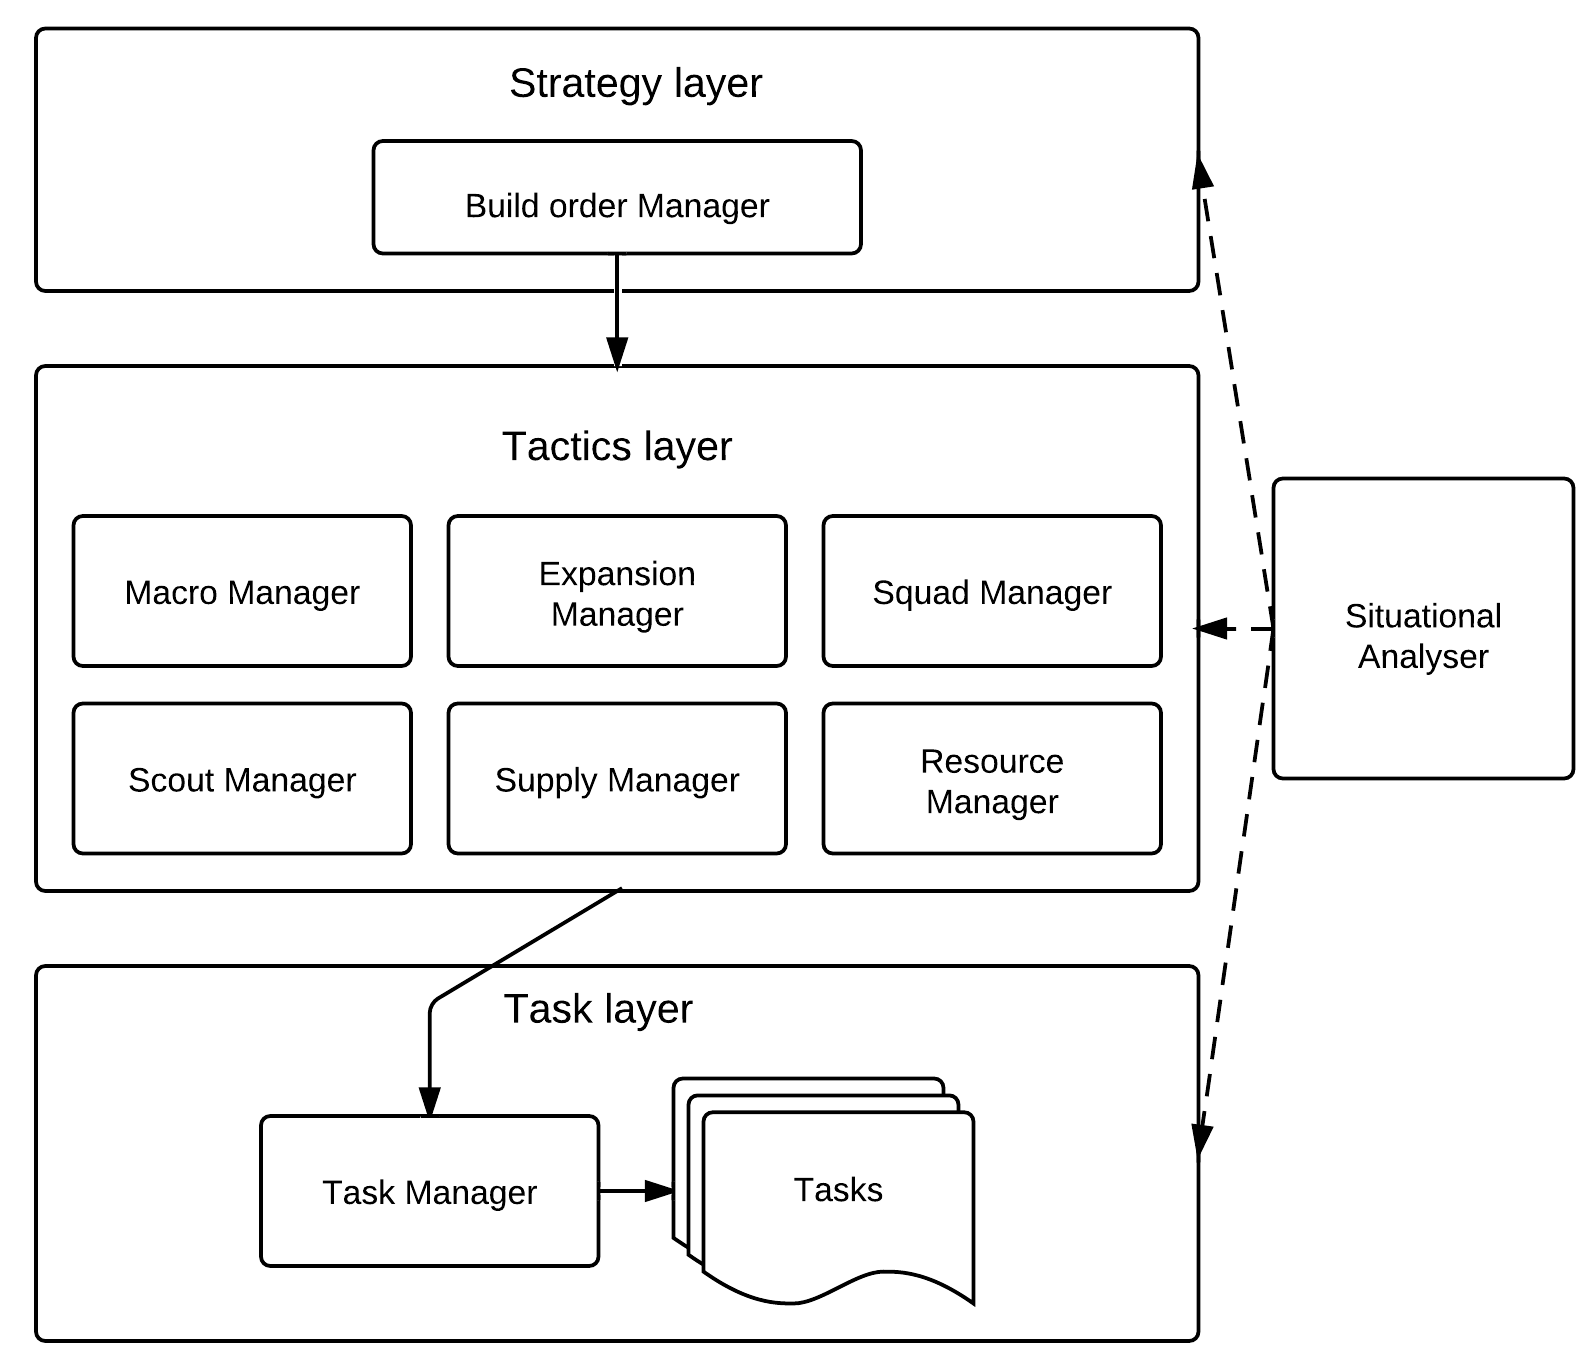
\includegraphics[scale=0.8]{graphics/skynet.png}
\caption{Skynet general architecture}
\label{fig:bthaiarch}
\end{figure}

\subsubsection{Nova}
Nova\cite{pérezmulti} has an architecture design that is quite close to BroodwarBotQ, except it uses a blackboard instead of an arbitrator. Nova is designed as a multi-agent system with managers and agents, and was design with that idea that having maximum possible information about the enemy at all times is essential for creating a good AI. Micro management is handled by abstraction, meaning you have a hierarchic system with general agents and the top, like the squad agent that is in charge of controlling an entire squad of units, and more specific agents at the bottom, like the Combat agent that handles fighting for the individual unit on the battlefield. Where as macro is handled with divide-and-conquer where a big problem is divided into smaller individual problems that each have a manager that tries to solve it. 

To achieve the initial goal of maximum information access the bot uses a blackboard for communication. Here all the modules can post data and intentions, and the other modules can then read this data. Anyone can read and write here, and all the information is available to every module that wants it. 

% TODO: maybe clear page here if that fits when report is done. 

\begin{figure}[h!tbp]
\centering
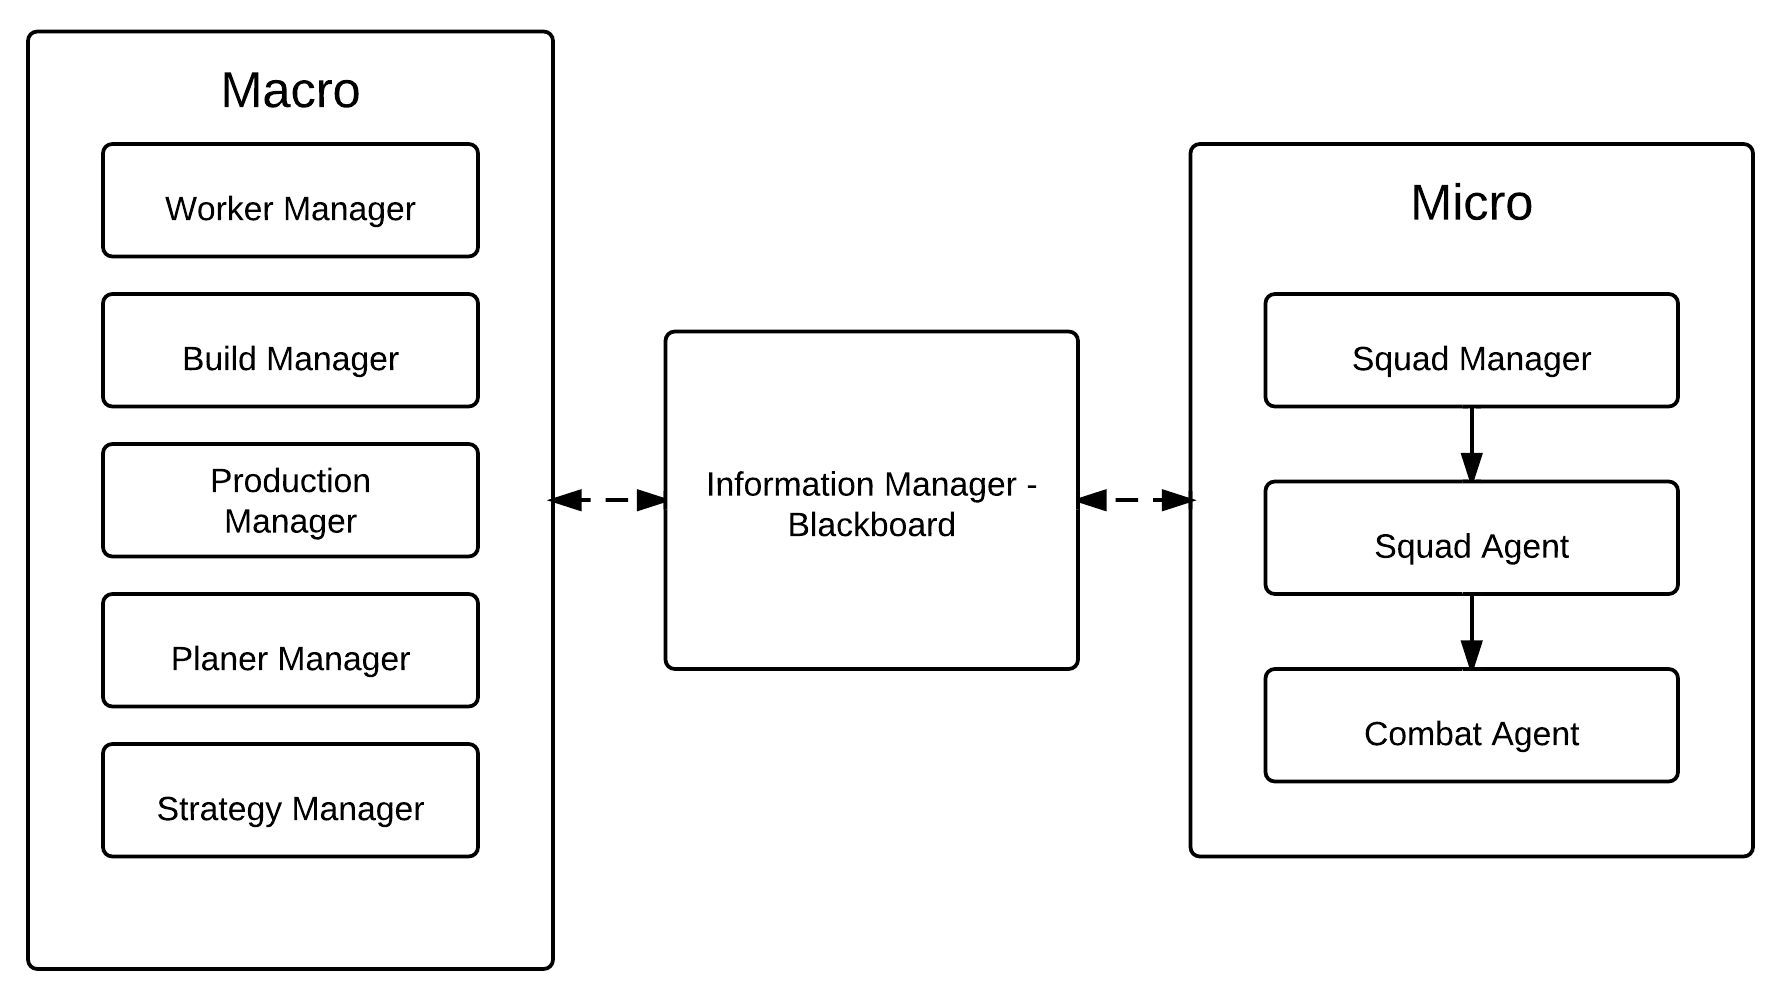
\includegraphics[scale=0.8]{graphics/nova.png}
\caption{Nova general architecture}
\label{fig:bthaiarch}
\end{figure}

\section{Cognitive Architectures}
Cognitive architectures are architectures that base themselves on some model of
human cognition. There are several competing models of cognition, and one of
the most recent and well-supported is the Global Workspace Theory.


One area that haven't been as well explored in relation to RTSes in general and
StarCraft in particular, is cognitive architectures, or models of cognition.
There has been some research done into implementing cognitive models for use in
first-person shooter games, but not into real-time strategy games. There
currently have been no attempts at utilizing cognitive models for playing
Starcraft: BroodWar. It would seem intuitive that real-time strategy games,
which have been considered a relatively hard problem to solve in a human-like
fashion, would benefit from using models based on our understanding of human
cognition.

\subsection{Models of cognition}
A cognitive model is an approximation of how cognitive processes work. They are
often used for understanding how humans take decisions, and predict 

\subsection{Global Workspace Theory}

Global Workspace Theory is a model of cognition that is very well supported
by experimental data and has been used to implement processes that imitate
human decision making (for example for solving the problem of assigning
people to jobs in the US Navy). 

It is based around an understanding of the brain as a set of many more or less
independent modules, working together by utilizing a shared workspace (hence the
``global workspace''), and cycles of the various submodules competing for a
space in this shared workspace.\cite{baars2005gwd}

\subsection{Cognitive Models in game AIs}
There have been several more or less successful attempts at implementing models
of cognition into game-playing agents. One of the more recent ones is
CERA-CRANIUM.


\subsection{CERA-CRANIUM}
CERA-CRANIUM intends to implement a general architecture for agents based on
various cognitive architectures, and not tied to any specific model of
cognition. It has already been used to implement a bot that plays Unreal
Tournament 2004 (a first-person shooter game) using a model based on the Global
Workspace Theory, as well as a robot for mapping out an unknown environment.
\cite{arrabales2009ceracranium}

It is based on two major modules:
\begin{description}
 \item [CRANIUM] (Cognitive Robotics Architecture Neurologically Inspired
Underlying Manager) is a tool to create and manage a large amount of
simultanous processes interacting through a shared workspace.
 \item [CERA] (Conscious and Emotional Reasoning Architecture)
 utilizes CRANIUM to create a dynamic control architecture structured in
layers, based on computational models of consciousness.
\end{description}

\subsubsection{CRANIUM}
CRANIUM is basically a software library that can execute thousand of parallel
but coordinated processes.
It is based on the understanding of how the brain works, where specialized
regions process information both from the senses and from other regions, and
the connections between these areas enables the emergence of the global
coordination we see in the brain.\cite{baars2005gwd}

In CRANIUM the various processes/modules are similar to the \textit{demons} in
Dennett's 1992 paper ``Consciousness Explained'', and CRANIUM itself is similar
to a \textit{pandemonium}\cite{dennet1992consciousness}.

The way the various processes collaborate on a shared workspace, by subscribing
to it, then read specific data from it, processing it and finally submitting the
new data back to the workspace is basically a blackboard
system.\cite{nii1986blackboard}

\subsubsection{CERA}
CERA is based around four layers; the sensory-motor services, physical layer,
mission-specific layer and the core layer, based on the services provided by
CRANIUM.

The sensory-motor layer is the most basic, and lowest-level layer, which
provides a uniform interface for sensory input and motoric actuation, physical
or simulated. Each sensor and motor has a service in this layer.

The physical layer wraps the sensory-motor layer, doing some pre-processing of
the sensory data, checking that actuator commands are within safety limits,
etc. It doesn't do semantic information binding, only simple, ``dumb''
pre-processing, though.

The mission-specific layer processes the data from the physical layer,
according to the current missions and sub-goals of those missions, as well as
vital behaviour of the bot (the inherent goals). The strict layering means that
this layer can be modified indendently of the other layers, to account for
various needs depending on the assigned tasks, and accounting for functional
integrity.

The core layer is the highest level, and perform higher cognitive functions,
and it is this layer that is adjusted to implement various cognitive
architectures. It has five core modules, however; attention, status assessment,
preconscious management, memory management and self-coordination. While these
are defined as core modules in CERA, the modular design means that they can be
replaced by a custom set.

The physical and mission-specific layers are inspired by cognitive models of
consciousness, where the various modules compete and collaborate in a shared
workspace. In CERA there is two workspaces; one for searching for the solution
to ``what must be the next content of the agent's conscious perception?'' and
``what must be the next action to execute?''. This differs from traditional AI
control architectures where one only attempts to find the best solution to the
second question, and ignoring the first. \cite{arrabales2009ceracranium} argues
that to successfully answer the second question in a human-like fashion, you
first need to answer the first one.

\subsubsection{Perceptual flow}
Perceptual flow is bottom-up, going from the physical sensors to the CERA core
layer. There are several types of percepts, depending on the level they are
produced in. The \textit{single percepts} are singular quantums of perceptions
directly from the percept pre-processors in the sensor service, \textit{complex
percepts} which are made from several individual single percepts, aggregated by
so-called ``percept aggregators''. These are specialized processors in the
physical layer who are responsible for noticing relations and contexts between
individual single percepts. These two types of percepts are both originating
from processors in the physical layer. From the specialized processors in the
mission-specific layer we get more abstract and complex percepts, who are also
more implementation specific. Some of the most important ones are
\textit{mission percepts}, \textit{complex percepts}, \textit{mismatch
percepts} and \textit{novelty percepts}, which say something about contexts for
the current focus of attention, activation, if some sensors input is not
matching the expected input, and the novelty of certain input.

Single percepts are published to the physical workspace, while combined, complex
percepts are published both to the physical workspace as well as the
mission-specific one, which means it becomes available to the specialized
processors in both layers immediately.

The percepts generated by the processors in the mission-specific layers
get published both to the mission-specific layer, as well as sent to the CERA
core layer. While using a single workspace would be possible, this decoupling
allows for a more modular and general design, where more of the architecture
can be re-used for different problems.

\subsubsection{Action flow}
Action flow is similar to perceptual flow, in that it gets conceptually simpler
the lower you go, and more complex and abstract further up in towards the core
layer. The flow is however top-down. From the processes in the mission-specific
layer comes \textit{mission behaviours}, which are decomposed into
\textit{simple behaviours} by action planners in the physical layer. These are
in turn unpacked into \textit{single actions}, by action pre-processors, which
can be executed by the motor services in the sensory-motor layer.

In the physical layer there is a action dispatcher, which is responsible for
dispatching individual actions to the motor services, according to the order
they come in, and the priority they are assigned from the processors they
originate in; as an example actions from simple behaviours with the highest
priority is executed before other actions from simple behaviours with lower
priority.

The selection of behaviours in the mission-specific layer is in turn controlled
by the core layer, and by mission goals.

\subsubsection{Feedback loops}
Looking at how percepts flow upwards from the sensory-motor layer, and back
down again, we can get a concept of \textit{feedback loops}, where different
kinds of events bounces from different layers in the system.

A feedback loop that only goes to the physical layer is compared to a reflexive
action, while loops that go through to the mission-specific layer and the core
layer respectively are compared to unconsciously performed actions and
higher-level conscious actions.

\subsubsection{Software architecture}
This model has a strong requirement on concurrency and asynchronous input and
output, and the software architecture reflects this. It is based on the
Microsoft Robotics Developer Studio, and the Concurrency and Coordination
Runtime in that, as well as the Decentralized Software Services, to implement a
light-weight distributed service-oriented architecture.

\subsubsection{Knowledge representation}
According to Arrabales\cite{arrabales2009ceracranium}, one of the key problems
in artificial general intelligence is knowledge representation. In CERA-CRANIUM
the knowledge is iteratively processed from the lower levels up to the core
layer, where lower layers contextualize and correlate input for higher level
processes. There is for example a proprioception module \footnote{Proprieception
is the knowledge of relative positions of ones own limbs.} which calculates the
position of exteroceptive sensors (sensors that observe external stimuli).
Knowledge is represented internally by geometrical vectors or integer variables,
referenced by contextual parameters referred to as $J$. Each percept is given a
$J$-index to define the relevant context it pertains to (for example geometric
position, or temporal position).

Handling conflicting and contradictory knowledge (which is very common in not
fully observable scenarious, with for example error-prone sensors) is given two
options; either assigning levels of confidence to the data itself and the
contextual parameters, or generating complex percepts representing the mismatch.

\subsubsection{Workspace modulation}
The core layer and the other layers are linked by the way which the
core layer can adjust the parameters by which the workspaces work. CRANIUM
creates a neural-like environment in which several processes can collaborate
and work towards a common goal, while CERA structures and controls the
collaboration in CRANIUM according to the cognitive architecture it models.

\subsubsection{Activation levels}
Cognitive architectures have a clear distinction betweeen implicit and explicit
processing\cite{atkinson2000consciousness}, and in CERA-CRANIUM all percepts
are by default implicit and get processed unconsciously. A specialized
competition inspired by the pandemonium model mentioned earlier selects the
conscious focus for explicit reasoning. The pandemonium demons are the
percepts, behaviours as well as the specialized processors. These are
constantly assigned an \textit{activation level} by the workspace, based on
input from the core layer.

The activation level is first used to weed out percepts with low activation
levels (to conserve computational power), and then the percepts with the highest
values are iteratively processed until one of them wins, and is selected as
conscious focus.

The specialized processors themselves are assigned more or less computational
power depending on their activation level. For specialized processors the
activation level is based on what input they can process.

At any given time there's also several different behaviours generated, and only
the ones with the highest activation level will be selected and executed.

\subsubsection{Contextualization}
The most important factor for the activation level for behaviours and percepts
is the contextualization criteria, which depends on a $J$-index sent to the
workspace from the core layer. The closer a behaviour or percepts own $J$-value
is to the current context $J$ from the core layer, the higher the activation
parameter it gets assigned. This means that percepts that are close to the
current context, and probably relevant for the problem at hand, will be more
likely to get chosen, and that behaviours that are directed at the current
context focus also will be more likely to be chosen.

Since the contextual bias influences which percepts are created, the perception
process is a very dynamic and active process, and not just a passive data
storage system.

\subsubsection{The Match/Mismatch/Novelty mechanism}
It also uses a mechanism to identify unexpected percepts, expected percepts and
novel percepts, and assigns higher activation values to these. This mechanism
was described by Pentti O. Haikonen in his 2007 book ``Robot Brains: Circuits
and Systems for Conscious Machines''\cite{haikonen2007robotbrains}. As an
example; a percept that doesn't match the predicted data will generate a
mismatch percept with an assigned high activation level because it might
require conscious attention. The core layer can then send a context command
with the appropriate $J$ context index to the workspaces to focus on the
unexpected percept.

\subsubsection{Core layer design}
One of the design goals of CERA-CRANIUM is that the higher cognitive abilities
should be problem domain independent.\cite{arrabales2009ceracranium} This means
that the core-layer is directed by meta-goals, instead of mission-specific ones.
This in turn means that different cognitive architectures (as in the models of
cognition, not software architectures) can be implemented on top of CERA-CRANIUM
in the core layer without having to change the lower levels. An example given by
Arrabales of a meta-goal is discovering abstractions, defined as detecting an
invariant in a variance.

\subsubsection{Goals}
Looking back at the different types of feedback loops (reflexive, unconscious,
and conscious), Arrabales identifies three types of goals;
\textit{basic-goals}, \textit{mission-goals} and \textit{meta-goals}, which are
achieved by their respective loops. While the basic and mission goals can be
kept constant for various cognitive architectures, the meta goals are dependent
on what kind of cognitive architecture the core layer is based on. The core
layer is therefore suited to model in higher cognitive features like emotions,
attention and imagination.

As an example, Arrabales implemented a core layer that continously calculates
a $J$-index and sends it with context commands to the workspaces to direct the
conscious focus. He relates this to the General Workspace Theory, where the
contexts generated are the outlines of the metaphorical ``spotlight'', and to
the Multiple Draft Model, where the core layer is in charge of selecting the
winning version, defined as the reduced set of percepts. His implementation is
rule based, where a set of rules takes in percepts and generates a new
$J$-index. These rules are based on the \textit{meta-goals}, and should
therefore, as explained earlier, be mission and domain independent.
%!TEX root = main.tex

\chapter{Results}

\section{Architecture}
\label{sec:architecture}

\subsection{The Game}
\subsubsection{JNI-BWAPI}
\subsection{Sensors and Controllers}
\subsubsection{Environment module}
\subsubsection{Sensor Memory module}
\subsubsection{Sensory-Motor module}

\chapter{Evaluation}
\section{Conclusion}
We have designed a modular architecture for a computer program that can play the
game StarCraft: Brood War, based on a cognitive architecture, emulating some of
the cognitive processes in the human mind. This was based on an exploration of
the problem of playing StarCraft: Brood War, a study of existing agents, and
also a review of relevant literature.

We have also briefly described some of the modules that would need to be
implemented in an agent.

\subsection{Evaluation of goals}
\subsubsection{Identify the most important aspects of a StarCraft match}
We have described the game play of a StarCraft: Brood War match, and what the
major problems are for an intelligent agent that wants to play it.
\subsubsection{Research existing solution and theories, using a structured
literature review}
The conclusion of the structured literature review lead to a large amount of
high-relevancy papers that needed to be read through, which we did, and then
selected what we thought was relevant to our paper.
\subsubsection{Design an architecture for a modular StarCraft playing computer
program}
Our previously described architecture is an attempt to bridge the domain of
real-time strategy games, and StarCraft: Brood War in particular, with the
model of cognitive processing that has been explored earlier.



\section{Evaluation}
Since we haven't implemented and tested the performance of our proposed
architecture, we have to rely on the testing done by others done in different
domains for estimating how efficient our agent will be. It is not given that the
single-focus approach taken by a cognitive architecture will be optimal for
something that would intuitively seem to require thinking about multiple things
at the same time. But we believe that the combination of unconscious processes
and the acknowledge-dispatch approach to handling threats and areas requiring
attention will lead to the agent being able to efficiently handle multi-pronged
problems.

\subsection{Evaluation of the structured literature review}
A large part of this project has been dedicated to the structured literature
review, henceforth referred to as the \textit{SLR}. While the SLR process went
mostly as planned, with few process-specific problems, the results were hugely
lacking and the process required an extraordinate amount of time.

The key problems we have identified were a lack of experience, lack of
leadership, lack of domain knowledge and a young domain.

The lack of experience should be fairly obvious, as SLR isn't very commonly
used in computer science. We were given an article on SLR that described the
process and need for it, but lack of practical experience among the
participants was very evident. For example was there disagreements on what
would constitute valid sources for articles, since a lot of relevant literature
was not published in peer-reviewed journals. The lack of
experience with SLR also lead to it taking a long time to concretize the goals
of the review itself into search terms.

The lack of leadership stemmed from being several independent groups with
independent goals (each group is graded individually). This meant that 12
individuals needed to argue to consensus for all decisions, since noone could
or would take on a leadership role.

Lack of domain knowledge was because a large part of the group had little to no
experience with neither the game itself (StarCraft) nor the design of software
architectures for game-playing agents. This meant that concretizing search
terms took much longer than needed, and that the search terms had to be decided
too early, before people had been able to read up on domain knowledge, which
lead to a sub-optimal searching process. This was partially reflected in the
results, because many of the highly rated articles were mostly useless.

Another problematic area is what we briefly touched on earlier, is that much of
the literature is not published in journals or academically recognized sources.
This is because StarCraft: Brood War agents is a relatively new area of
research, and many of the participants are simply programmers who do this for
fun in their spare time. This means that much of the literature describing the
state of the art simply doesn't exist, or only exists as blog posts or similar.
This makes searching for relevant literature hard when one has to stay within
the relatively strict boundaries defined by the SLR. On the other hand,
research into cognition is also a relatively young interest field, and the
amount of recent and valuable literature regarding about is not impossible for a
single person to sift through, and it would have been more efficient than
splitting up the work like with the SLR. The indication for this is that only a
handful of the relevant papers we based our eventual report on turned up in the
SLR, and all the relevant papers that turned up in the SLR we were familiar
with beforehand.


\section{Impact}
We believe that using cognitive models is interesting both from a
game-development perspective, for more realistic and engaging gameplay, as well
as from a purely academic viewpoint, furthering the understanding of cognitive
models, and giving researchers yet another environment and domain in which to
test cognitive models.

\section{Future work}
The biggest part remaining is to actually implement this architecture, and see
if it is viable. This will include more closely detailing the various
specialized processors in each layer, as well as elaborating on the meta-goals
for the core layer, and implementing a rule set to describe these.

Another important extension would be to more tightly integrate learning into
the architecture. Inspiration for how to do this could possibly be done by
looking at how it is implemented in the LIDA model\cite{franklin2007lida}.
\endrefsection
\printbibliography[segment=0]


%%!TEX root = main.tex
% Appendix
\appendix
\begin{refsegment}

\chapter{Structured Literature Review}
\label{appendix:slrreport}

% Review these, could probably remove \slrMadeBy
\newcommand{\slrTitle}{Structured Literature Review}
\newcommand{\slrSubtitle}{Fall project 2011}
\newcommand{\slrMadeby}{Magnus Sellereite Fjell, Stian Veum M{\o}llersen, Tobias Laupsa Nilsen, J{\o}rgen B{\o}e Svendsen, Espen Auran Rathe, Aleksander Lun{\o}e Waage, Martin Tobias Holmedahl Sandsmark, Ken B{\o}rge Melhus Viktil, {\O}ystein Samuelsen, Finn Robin K{\aa}veland Hansen, Dag-{\O}yvind Tornes and Jan Eriksson}
\newcommand{\slrDate}{December 2011}
\newcommand{\Hline}{\rule{\linewidth}{0.3mm} \\}

\begin{center}
\large \textbf{\slrMadeby}

\vspace{3cm}
\Hline
\Huge \textsc{\slrTitle}
\vspace{2cm}
\huge \\ \textsc{\slrSubtitle}
\Hline
\vfill
\normalsize \slrDate
\end{center}

\section{Introduction}
%!TEX root = main.tex

\chapter{Introduction}

\section{Background and motivation}

\subsection{The Problem}
In 2003 Michael Buro published an article where he requested more artificial
intelligence research in the domain of real-time strategy
games.\cite{buro2003real} Before this, a lot of research was focused mainly on
turn based, real-time board games, like chess and checkers. A lot of
progress has been done in these fields to the point where they are now able to
beat top level human players in a real-time match. \cite{campbell2002deep} But
these games are both deterministic and fully observable, whereas real-time
strategy games usually are only partially deterministic and partially
observable, which makes for much more interesting problems.

In the wake Buro's call to arms more work has been invested in this area, and
several platforms for RTS research has been used. One platform that has been
used a lot is Wargus\cite{wargus}, a clone of Blizzard's Warcraft 2, where they
created a Lua-based AI scripting language for efficient artificial game-playing
agent creation. But this game had quite severe limitations on individual
management of units, so in recent years StarCraft: Brood War has been getting a
lot more attention as a platform for experimenting with game playing agents.
Several competitions are held each year where implemented AI agents can
compete with each other and measure their performance. But even though a lot has
happened with the field in recent years, Starcraft agents still have ways to go
before they can measure up to a human player.\cite{eisbotvsfong}.

Simply winning is however not always the goal, most game-playing artificial
intelligences are made to be realistic and engaging to compete with, so in many
situations simply playing well is not enough. According to Arrabales et
al \cite{arrabales2009gamechars} it is still more realistic and engaging to be
playing with other humans than with synthetic agents. So to attempt to lessen
this gap, it could be interesting to make synthetic agents play more human-like,
and to do this one would probably want to look into more biologically inspired
methods, for example inspired by cognitive architectures.

Cognitive architectures have proven to lead to human-like behaviour and choices
in both games\cite{arrabales2009gamechars} and general problem
solving\cite{franklin2003interacting}, and the logical conclusion therefore
seems to be to try to apply these models to StarCraft.

\subsection{StarCraft: Brood War and BWAPI}
StarCraft is one of the most popular real-time strategy games in the world. It
was developed by Blizzard Entertainment, and in 1998 they released the expansion
pack Brood War. The expansion pack included new maps, units and upgrades for
each of the races in the game.
 
Since its release it has been widely played in professional tournaments, as well
as been used extensively in research on artificial intelligence, thanks to the
BWAPI project which is a free software project aimed at developing and
maintaining an API, named BWAPI, for creating artificial intelligence modules
for Brood War. In addition, this API is the basis for several yearly
competitions where people can submit AI bots that will be pitted against other
bots to measure their relative performance. This has led to a large number of
AIs being developed of various degrees of complexity and novelty, both from
researchers and hobby developers. 

\subsection{The project}
In this project we will familiarize ourselves with the game StarCraft: Brood
War, and what challenges that presents when creating a computer program that
will play the game. We will identify the different aspects of a StarCraft game
that are important to solve in order to create a good game-playing agent, and
also look at how other researchers have solved these problems in their agents.
Ultimately we will select and define an architecture for our system that will
have an modular approach in order to support easier collaboration when
implementing the system, based on a cognitive model.

In order to get a good overview of existing solutions and map the current state
of the research into this field, we will perform a structured literature review.
This will give us a good overview of the theory behind the state of the art
when it comes to our research problem.

So our project is divided into three main parts:
\begin{enumerate}
  \item Identify the most important aspects of a StarCraft match.
  \item Research existing solution and theories, using a structured literature
review.
  \item Design an architecture for a modular StarCraft playing computer
program, based on a cognitive model.
\end{enumerate}

\section{Contributions}
For the structured literature review we collaborated with Magnus Sellereite
Fjell, Stian Veum M{\o}llersen, Tobias Laupsa Nilsen, J{\o}rgen B{\o}e Svendsen,
Espen Auran Rathe, Aleksander Lun{\o}e Waage, {\O}ystein Samuelsen, Finn Robin
K{\aa}veland Hansen, Dag-{\O}yvind Tornes and Jan Eriksson.

We are also grateful for the feedback and cooperation with everyone on the
\#BWAPI IRC channel on QuakeNet, and especially Adam Heinermann who is also a
lead developer on the BWAPI project.

We would also like to thank our supervisors; Helge Langseth, Anders
Kofod-Petersen and Pauline Haddow.

\section{Report Structure}
This report is structured into four chapters:
\begin{itemize}
\item Chapter 1: \textbf{Introduction} \\
This chapter describes the motivation and goal of the project as well as who contributed and the general structure of the report.
\item Chapter 2: \textbf{Theory} \\
This chapter is threefold. First it presents some theory on StarCraft in
general, how the most important mechanics works and the difference between the
available races. Then we go over the state of the art when it comes to agents
who play StarCraft, both how the problems they solve are partitioned, as well
as how some of the most important agents today are architected. Lastly we go
over some background on the current state of cognitive research and models
utilizing this.
\item Chapter 3: \textbf{Results} \\
Here we present our results; our novel architecture for an agent for playing
StarCraft: Brood War based on the cognitive models we explored earlier.
\item Chapter 4: \textbf{Evaluation} \\
Here we summarize and evaluate the work presented in this report.




\end{itemize}

\section{Structured Literature Review}
\input{slr-scbw/sections/about_slr}

\section{Protocol and Procedure}
\input{slr-scbw/sections/protocol}

\section{Search Engines and Search Strings}
\input{slr-scbw/sections/search_engines}

\section{Search Results}
\input{slr-scbw/sections/search_results}

\section{Score Sheet}
\input{slr-scbw/sections/score_sheet}

\clearpage

\end{refsegment}

\cleardoublepage
\phantomsection
\pagestyle{plain}
\addcontentsline{toc}{section}{Structured Literature Review - Bibliography}
\printbibliography[segment=1, title=Structured Literature Review - Bibliography]



\end{document}
